\documentclass[11pt,paper=a4,answers]{exam}
\usepackage{graphicx,lastpage}
\usepackage{upgreek}
\usepackage{hyperref}
\usepackage{amsmath}
\usepackage{enumerate}
\usepackage{censor}
\usepackage{amsmath,amssymb,amsfonts}
\usepackage{tcolorbox}
\usepackage[utf8]{inputenc}
\usepackage{array}
\usepackage{adjustbox} % For adjusting and aligning content
\usepackage{listings}
\usepackage{color}
\usepackage{hyperref}
\usepackage{multicol}
% Package for coloring text
\usepackage{xcolor}

% Define a very light gray color
\definecolor{verylightgray}{rgb}{0.95,0.95,0.95}

% Define styles for listings
\lstdefinestyle{cppStyle}{
    language=C++,
    basicstyle=\ttfamily\small, % Change to \tiny for smaller text
    keywordstyle=\color{blue},
    commentstyle=\color{green},
    stringstyle=\color{red},
    numbers=left,
    numberstyle=\tiny\color{gray},
    stepnumber=1,
    numbersep=5pt,
    backgroundcolor=\color{verylightgray}, % Use the very light gray color
    frame=single,
    rulecolor=\color{black},
    showstringspaces=false
}

% Define for C
\lstdefinestyle{cStyle}{
    language=C,
    basicstyle=\ttfamily\small, % Change to \tiny for smaller text
    keywordstyle=\color{blue},
    commentstyle=\color{green},
    stringstyle=\color{red},
    numbers=left,
    numberstyle=\tiny\color{gray},
    stepnumber=1,
    numbersep=5pt,
    backgroundcolor=\color{verylightgray}, % Use the very light gray color
    frame=single,
    rulecolor=\color{black},
    showstringspaces=false
}

\lstdefinestyle{asmStyle}{
    language=[x86masm]Assembler,
    basicstyle=\ttfamily\small, % Change to \tiny for smaller text
    keywordstyle=\color{black},
    commentstyle=\color{green},
    stringstyle=\color{red},
    numbers=left,
    numberstyle=\tiny\color{gray},
    stepnumber=1,
    numbersep=5pt,
    backgroundcolor=\color{verylightgray}, % Use the very light gray color
    frame=single,
    rulecolor=\color{black},
    showstringspaces=false
}

% Define for python
\lstdefinestyle{pythonStyle}{
    language=Python,
    basicstyle=\ttfamily\small, % Change to \tiny for smaller text
    keywordstyle=\color{blue},
    commentstyle=\color{green},
    stringstyle=\color{red},
    numbers=left,
    numberstyle=\tiny\color{gray},
    stepnumber=1,
    numbersep=5pt,
    backgroundcolor=\color{verylightgray}, % Use the very light gray color
    frame=single,
    rulecolor=\color{black},
    showstringspaces=false
}

% Define for java
\lstdefinestyle{javaStyle}{
    language=Java,
    basicstyle=\ttfamily\small, % Change to \tiny for smaller text
    keywordstyle=\color{blue},
    commentstyle=\color{green},
    stringstyle=\color{red},
    numbers=left,
    numberstyle=\tiny\color{gray},
    stepnumber=1,
    numbersep=5pt,
    backgroundcolor=\color{verylightgray}, % Use the very light gray color
    frame=single,
    rulecolor=\color{black},
    showstringspaces=false
}

% Define for java bytecode
\lstdefinestyle{bytecodeStyle}{
    language=Java,
    basicstyle=\ttfamily\small, % Change to \tiny for smaller text
    keywordstyle=\color{blue},
    commentstyle=\color{green},
    stringstyle=\color{red},
    numbers=left,
    numberstyle=\tiny\color{gray},
    stepnumber=1,
    numbersep=5pt,
    backgroundcolor=\color{verylightgray}, % Use the very light gray color
    frame=single,
    rulecolor=\color{black},
    showstringspaces=false
}

\censorruledepth=-.2ex
\censorruleheight=.1ex
\hyphenpenalty 10000
\usepackage[paperheight=10.5in,paperwidth=8.27in,bindingoffset=0in,left=0.8in,right=1in,
top=0.7in,bottom=1in,headsep=.5\baselineskip]{geometry}
\flushbottom
\usepackage[normalem]{ulem}
\renewcommand\ULthickness{1pt}
\setlength\ULdepth{1.5ex}
\renewcommand{\baselinestretch}{1}
\pagestyle{empty}
\hypersetup{
    colorlinks=true,
    linkcolor=blue,
    filecolor=magenta,      
    urlcolor=blue,
    pdftitle={Just-In-Time Compilation: Part 1}
    }
\pagestyle{headandfoot}
\headrule

\runningheader{\footnotesize}
{Just-In-Time Compilation: Part 1}
\footrule
\footer{\footnotesize}
{\hrule width \textwidth height 1pt \vspace{1mm} Page \thepage\ of \numpages}
{}

\pointsinrightmargin
\pointsdroppedatright
\marksnotpoints
\marginpointname{ \points}
\pointformat{\boldmath\themarginpoints}

\begin{document}

\thispagestyle{empty}

\begin{tcolorbox}[colback=blue!10!white, colframe=gray!20!blue, width=\textwidth, boxrule=0.5mm, arc=0mm, auto outer arc]
    \begin{tabular*}{\textwidth}{@{\extracolsep{\fill}} l r}
        \textbf{CS60203: Design Optimization of Computing Systems} & \textit{\today} \\
    \end{tabular*}
    \begin{center}
        \textbf{\LARGE Just-In-Time Compilation: Part 1} \\
    \end{center}
    \begin{tabular*}{\textwidth}{@{\extracolsep{\fill}} l r}
        \textit{Instructor: Mainack Mondal} & \textit{Scribe-By:  Bratin Mondal } \\
    \end{tabular*}
\end{tcolorbox}

\vspace{2mm}

\noindent
Just-In-Time (JIT) compilation is a technique that improves the runtime performance of a program by compiling the code at runtime. The compiled code is then executed instead of the original code. This technique is used in many modern programming languages and runtime environments. This scribe describes the tradeoffs of using interpreted and compiled languages and the benefits of JIT compilation along with addressing the critical question \textbf{To JIT or not to JIT ?} 

\section{Interpreted vs Compiled Languages}
\subsection{Compiled Languages}
\textit{Compilation of source code into object code by the compiler.} Classic examples of compiled languages are C, C++, and Fortran. The source code is compiled into object code, which the processor executes. The compiled code is usually faster than the interpreted code because it is optimized for the target architecture although generating such optimized code takes significant time. Simply put, the more optimizations the compiler does, the more time it will take.

\begin{tcolorbox}
    \href{https://stackoverflow.com/questions/466790/assembly-code-vs-machine-code-vs-object-code}{\textbf{Machine Code vs Object Code:}}
    Machine code is binary code (1's and 0's) that the CPU can execute directly, appearing as unprintable characters in a text editor. Object code, a subset of machine code, represents a module or library and contains placeholders or offsets for linking, which the linker resolves to create a complete program.
 \end{tcolorbox}

\subsection{Interpreted Languages}
\textit{In computer science, an interpreter is a computer program that directly executes instructions written in a programming or scripting language without requiring them previously to have been compiled into a machine language program.} Classic examples of interpreted languages are Python, Ruby, and JavaScript. Essentially, interpreter is a program that consumes a series of instructions and executes them against an abstract machine.

\subsection{Why Interpreters?}
\subsubsection{Platform Independence}
Consider the C++ code snippet below:
\begin{lstlisting}[style=cppStyle]
    int square(int num) {
        return num * num;
    }
\end{lstlisting}
When compiled, this code is specific to the target architecture. Consider the x86-64 assembly code on the left and the ARM assembly code on the right. The architectures use their respective instruction sets, and the compiled code is not portable across architectures and needs to be recompiled every time from the source code.

\begin{adjustbox}{valign=t,minipage=0.52\textwidth}
    \textbf{x86-64 assembly code}
    \begin{lstlisting}[style=asmStyle]
        square(int):
        push    rbp
        mov     rbp, rsp
        mov     DWORD PTR [rbp-4], edi
        mov     eax, DWORD PTR [rbp-4]
        imul    eax, eax
        pop     rbp
        ret
    \end{lstlisting}
\end{adjustbox}
\hfill
\begin{adjustbox}{valign=t,minipage=0.42\textwidth}
    \textbf{ARM assembly code}
    \begin{lstlisting}[style=asmStyle]
        square(int):
        push    {r7}
        sub     sp, sp, #12
        add     r7, sp, #0
        str     r0, [r7, #4]
        ldr     r3, [r7, #4]
        mul     r3, r3, r3
        mov     r0, r3
        adds    r7, r7, #12
        mov     sp, r7
        ldr     r7, [sp], #4
        bx      lr
    \end{lstlisting}
\end{adjustbox}

Now consider the Java code and the corresponding bytecode. The Java code is compiled into bytecode, which is executed by the Java Virtual Machine (JVM). The JVM is platform-independent, and the bytecode is portable across architectures.

\begin{adjustbox}{valign=t,minipage=0.43\textwidth}
    \textbf{Java code}
    \begin{lstlisting}[style=javaStyle]
class Square {
    static int square(int num) {
        return num * num;
    }
}
    \end{lstlisting}
\end{adjustbox}
\hfill
\begin{adjustbox}{valign=t,minipage=0.52\textwidth}
    \textbf{Bytecode}
    \begin{lstlisting}[style=bytecodeStyle]
class Square {
    Square();
            0: aload_0
            1: invokespecial #1                  // Method java/lang/Object."<init>":()V
            4: return
    
    static int square(int);
            0: iload_0
            1: iload_0
            2: imul
            3: ireturn
    
    }
    \end{lstlisting}
\end{adjustbox}


\subsubsection{Runtime Type Information}
\textit{Runtime Type Information (RTTI) is a mechanism that allows the type of an object to be determined at runtime.} This is crucial for advanced features like dynamic types, dynamic dispatch, and reflection. A classic example is \texttt{PyTypeObject} in Python, a C structure used to describe the built-in types of Python objects. \texttt{PyTypeObject} contains fields such as the type name, object size, memory allocation methods, and function pointers for operations like printing, comparing, and hashing. This structure is central to Python's type system, enabling efficient type checking and method dispatch at runtime. For more details, refer \href{https://docs.python.org/3/c-api/type.html#c.PyTypeObject}{here}.

\subsubsection{Reflection}
Reflection is the ability of a program to examine and modify its own structure and behavior at runtime. 
\textit{Source code that “introspects” / “manipulates” source code.} As an example, consider the Java code snippet below:
\begin{lstlisting}[style=javaStyle]
import java.lang.reflect.*;

public class DumpMethods {
    public static void main(String[] args) {
        try {
            Class c = Class.forName(args[0]);
            Method m[] = c.getDeclaredMethods();
            for(int i = 0; i < m.length; i++)
                System.out.println(m[i].toString());
        } catch(Throwable e) {
            System.err.println(e);
        }
    }
}
\end{lstlisting}
 The \texttt{Class.forName()} method is used to load the class, and the \texttt{getDeclaredMethods()} method is used to get the methods of the class. The code snippet prints the methods of the class passed as an argument. Such information can be very useful for enabling developers to inspect and interact with classes and objects at runtime, which is essential for building frameworks, debugging tools, and dynamic proxies. This approach is compelling in scenarios where the class to be inspected is not known until runtime.

 \tcbset{
    colback=gray!20,         % Background color
    colframe=black,          % Border color
    boxrule=0.5mm,           % Border thickness
    arc=2mm,                 % Rounded corners
    boxsep=1pt,              % Separation between box and content
    fontupper=\small,        % Font size inside the box
}

 \begin{tcolorbox}
    \href{https://stackoverflow.com/questions/359237/why-does-c-not-have-reflection}{\textbf{Reflection and C++:}} There are many reasons why C++ does not have reflection. 
    \begin{itemize}
        \item \textbf{You don't pay for what you don't use:} Implementing reflection would require to store metadata about classes and methods whereas the programmer might never need them and it's totally an overhead.
        \item \textbf{Complier Optimization:} The C++ compiler often does agressive optimizations which consists of inlining functions, removing dead code, etc. As a result, it might be the case that a class or method is not even present in the final executable. With reflection, the compiler would have to store metadata about all classes and methods which would be a waste of space.


 \item \textbf{Template Metaprogramming:}
 Every template instantiation is a new type in C++. Alongside this, it can create other types and functions. For example consider declaring \texttt{std::vector<int>}. At such situations, we would also expect to see \texttt{std::vector<int>::iterator} in reflection system.  If the program never actually uses this iterator class template, its type will never have been instantiated, and so the compiler won't have generated the class in the first place. And it's too late to create it at runtime, since it requires access to the source code.
 \item \textbf{Alternative to Reflection:} Reflection isn't as vital in C++ as it is in languages like C\#. The reason is template metaprogramming, which, while not a replacement for everything, can achieve many of the same goals at compile-time. For instance, the \texttt{boost::type\_traits} library allows for querying type information that, in languages like C\#, would typically require reflection. 
 \end{itemize}
 \href{https://www.open-std.org/jtc1/sc22/wg21/docs/papers/2023/p2996r0.html}{\textbf{Reflection in C++ 26}} - a proposal to add reflection to C++.
\end{tcolorbox}

\subsubsection{Additional runtime accessible information}\label{sec:runtime}
Interpreted languages can contain code as a runtime object also.

For example Python has \href{https://github.com/python/cpython/blob/main/Python/assemble.c} {\texttt{PyCodeObject}} that wraps the bytecode and other information about the code. This C structure of the objects is used to describe the code objects. It has different fields and methods like \texttt{co\_code} which is the bytecode, \texttt{co\_consts} which is the tuple of constants used in the code, \texttt{co\_varnames} which is the tuple of variable names used in the code, \texttt{PyCode\_GetNumFree()} which returns the number of free variables used in the code, etc.
 For more details, refer \href{https://docs.python.org/3/c-api/code.html}{here}.
\subsubsection{Instrumentation}
For interpreted languages, the runtime information can be used to instrument the code in case of unexpected behavior. Furthermore, we can measure other metrics like the number of times a function is called, the time taken by a function, etc. The runtime information can be used to profile the code line-by-line and inspect the program state. Python runtime also has Instrumentation using \href{https://github.com/python/cpython/blob/main/Include/cpython/code.h}{\texttt{\_Py\_*\_Monitors}}. 

In compiled languages, instrumentation is more challenging due to code being transformed into machine code, losing high-level details. This makes inserting instrumentation points harder and may impact performance, requiring tools like profilers to assist with analysis.


% Increase the size of the font in the tcolorbox
\begin{tcolorbox}[fontupper=\large]
    % Center
    \begin{center}
        % Write in green
        \textcolor{green}{\textbf{Interpreters are Nice}} \\
        \textcolor{red}{\textbf{Interpreters can be Slow}}
    \end{center}
\end{tcolorbox}

\subsection{CPython vs Cython}
Cython uses almost the same syntax as Python, but it is a compiled language. Cython compiles python code into C code using \href{https://docs.python.org/3/c-api/}{C/Python API} and then compiles and executes the C code. Cython is faster than Python because it is compiled, but it is slower than C because it is a higher-level language.

Consider the Python code snippet below, which multiplies two matrices:
\begin{lstlisting}[style=pythonStyle]
def matmul(A, B, out):
    for i in range(len(A)):
        for j in range(len(B[0])):
            s = 0
            for k in range(len(B)):
                s += A[i][k] * B[k][j]
            out[i][j] = s
\end{lstlisting}

\subsubsection{Simple Compilation}
Direct compilation of the Python code using Cython generates the \href{https://pastebin.com/CeV1ZBxS}{C code}. For simpler understanding, let's analyze the \texttt{A[i, k]} part of the code. It gets converted to:
\begin{lstlisting}[style=cStyle]
tmp = PyTuple_New(2);
if (!tmp) { err_lineno = 21; goto error; }
Py_INCREF(i);
PyTuple_SET_ITEM(tmp, 0, i);
Py_INCREF(k);
PyTuple_SET_ITEM(tmp, 1, k);
A_ik = PyObject_GetItem(A, tmp);
if (!A_ik) { err_lineno = 21; goto error; }
Py_DECREF(tmp);
\end{lstlisting}    
Direct compilation makes the code only \textbf{1.15x} faster than the CPython. It has two major limitations:
\begin{itemize}
    \item The code is still using the Python API to lookup Python objects, which is slow.
    \item The code is still using \texttt{PyNumber\_Multiply} to multiply two Python objects, which is slow.
\end{itemize}

\subsubsection{Using NumPy}
The fact that type of the variables is not known at compile time is a major limitation. Instead, let's define A and B as NumPy arrays and use the NumPy API to access the elements. Consider the code snippet below:
\begin{lstlisting}[style=pythonStyle]
import numpy as np
cimport numpy as np
ctypedef np.float64_t dtype_t

def matmul(np.ndarray[dtype_t, ndim=2] A,
           np.ndarray[dtype_t, ndim=2] B,
           np.ndarray[dtype_t, ndim=2] out=None):
    cdef Py_ssize_t i, j, k
    cdef dtype_t s\usepackage{emoji}
    if A is None or B is None:
        raise ValueError("Input matrix cannot be None")
    for i in range(A.shape[0]):
        for j in range(B.shape[1]):
            s = 0
            for k in range(A.shape[1]):
                s += A[i, k] * B[k, j]
            out[i,j] = s
\end{lstlisting}
On compiling the above code, the \href{https://pastebin.com/28jYiVf2}{C code} generated is much more optimized. The code is \textbf{180-190x} faster than the CPython. Again, let's analyze the \texttt{A[i, k]} part of the code. It gets converted to:
\begin{lstlisting}[style=cStyle]
tmp_i = i; tmp_k = k;
if (tmp_i < 0) tmp_i += A_shape_0;
if (tmp_i < 0 || tmp_i >= A_shape_1) {
    PyErr_Format(...);
    err_lineno = 33; goto error;
}
if (tmp_k < 0) tmp_k += A_shape_1;
if (tmp_k < 0 || tmp_k >= A_shape_1) {
    PyErr_Format(...);
    err_lineno = 33; goto error;
}
A_ik = *(dtype_t*)(A_data + tmp_i * A_stride_0 + tmp_k * A_stride_1);
\end{lstlisting}
The usage of NumPy arrays and the NumPy API makes the code much faster than the CPython as the lookup of the elements is done using the NumPy API which is faster.
\subsubsection{Removing Bound Checks}
One of the major reasons for the slowdown of the code is the bound checks for the Matrices. We add the following lines to remove the bound checks:
\begin{lstlisting}[style=pythonStyle]
import cython
@cython.boundscheck(False)
@cython.wraparound(False)
\end{lstlisting}
The \href{https://pastebin.com/emJDYFkM}{C code} generated is \textbf{700-800x} faster than the CPython. Although we have now compromised on the safety of the code, the code is much faster than the CPython. So, compilation of code earlier can significantly reduce execution time.


\section{Just-In-Time Compilation}
\textit{Just-In-Time compilation is compilation (of computer code) during execution of a program (at run time) rather than before execution. This may consist of source code translation but is more commonly bytecode translation to machine code, which is then executed directly.} Before we move forward with JIT, recall that Interpreted languages can also contain code as a runtime object as discussed in Section \ref{sec:runtime}.

\subsection{What is JIT?}

\begin{figure}[h]
    \centering
    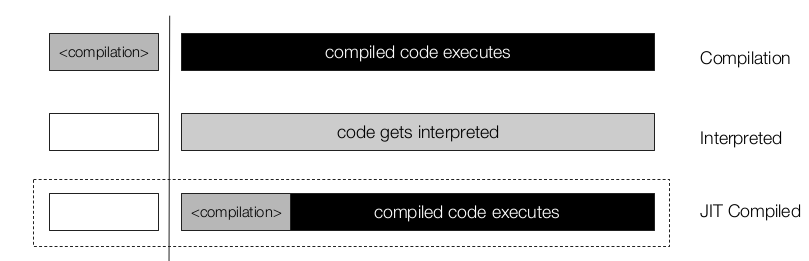
\includegraphics[scale=0.44]{Extras/JIT.png}
    \caption{Compilation vs Interpretation vs JIT Compilation}
    \label{fig:your_label}
\end{figure}
Just-In-Time (JIT) compilation converts source or bytecode into machine code at runtime. The compiled code is stored in memory, optimized for the target architecture, and can be executed repeatedly, making it faster than interpreted code. The JIT compiler can also optimize the code based on runtime information, making it faster than compiled code.Interpreted languages get executed line-by-line (or instruction-by-instructions) hence it is possible to only compile parts of the code and interpret the rest
\subsection{To JIT or not to JIT ?}
\subsubsection{Startup Time vs Execution Time Tradeoff}
Start-up time is the time taken by the JIT compiler to produce the machine code.
Execution time is time taken by the machine code to execute.

Interpreters have low start-up time but high execution time. Compiled languages have high start-up time but low execution time. Using sophisticated compilers can produce optimized machine code but it is a time-consuming process which delays the start-up. For JIT it is essential to consider the use-case. For example in a Real-Time Data Processing System such as stock trading algorithms, the start-up time is not a concern but the execution time is. In such cases, JIT might not be a good choice. On the other hand, for command-line tools, the start-up time is a concern but the execution time is not so much. In such cases, JIT might be a good choice.
\begin{figure}[h]
    \centering
    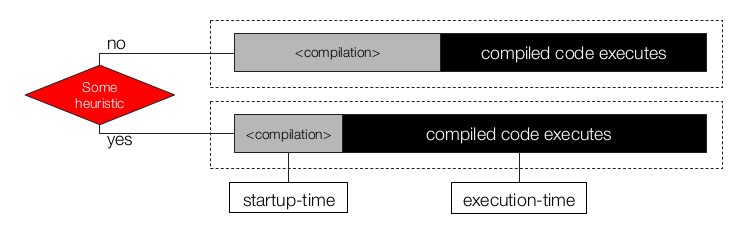
\includegraphics[scale=0.49]{Extras/STARTUP_VS_EXECUTION.png}
    \caption{Compilation vs Interpretation vs JIT Compilation}
    \label{fig:your_label}
\end{figure}
\subsubsection{Memory Requirements Tradeoff}
Interpreters require less memory as they do not store the compiled code. Compiled languages require more memory as they store the compiled code.

JIT requires significant memory as it stores the compiled code. Moreover using a simpler compiler may reduce the start-up time but produces unoptimized larger code. Using a sophisticated compiler may reduce the execution time but produces optimized smaller code. It is a design tradeoff between the start-up time, execution time, and memory requirements.
\begin{figure}[h]
    \centering
    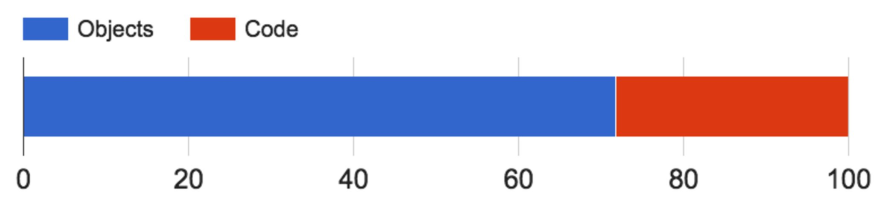
\includegraphics[scale=0.26]{Extras/V8_HEAP.png}
    \caption{\href{https://docs.google.com/presentation/d/1chhN90uB8yPaIhx_h2M3lPyxPgdPmkADqSNAoXYQiVE/edit?usp=sharing}{V8 heap usage by code-objects}}
    \label{fig:your_label}
\end{figure}

%  Section without number
% \section*{References}
% %  List all the references used in the document
% \begin{enumerate}
%     \item \href{https://stackoverflow.com/questions/466790/assembly-code-vs-machine-code-vs-object-code}{Assembly code vs Machine code vs Object code} - A Stack Overflow discussion on Assembly code vd Machine Code vs Object Code
%     \item \href{https://docs.python.org/3/c-api/type.html#c.PyTypeObject}{Python Type Object} - Documentation on the `PyTypeObject` structure, which represents Python types in the C API.
%     \item \href{https://stackoverflow.com/questions/359237/why-does-c-not-have-reflection}{Reflection in C++} - A Stack Overflow discussion explaining why C++ does not natively support reflection.
%     \item \href{https://www.open-std.org/jtc1/sc22/wg21/docs/papers/2023/p2996r0.html}{Reflection in C++ 26} - Proposal for adding reflection capabilities to C++.
%     \item \href{https://docs.python.org/3/c-api/code.html}{Python Code Object} - Documentation on the `PyCodeObject` structure, which represents code objects in Python's C API.
%     \item \href{https://github.com/python/cpython/blob/main/Include/cpython/code.h}{Python Monitors} - Instrumentation in Python using `\_Py\_*\_Monitors`. 
%     \item \href{https://docs.python.org/3/c-api/}{C/Python API} - Overview of the C API for Python, including functions and structures for interfacing with Python from C.
%     \item \href{https://docs.google.com/presentation/d/1chhN90uB8yPaIhx_h2M3lPyxPgdPmkADqSNAoXYQiVE/edit?usp=sharing}{V8 heap usage by code-objects} - A Google Slides presentation detailing V8's heap usage and management for code objects by Leszek Swirski \& Ross McIlroy.    
% \end{enumerate}

\begin{thebibliography}{9}
    \bibitem{mainack}

    \href{https://kronos-192081.github.io/DOCS-2024/slides/T03_JIT.pdf} {Just-In-Time Compilation: Part 1} - Lecture slides on Just-In-Time Compilation: Part 1 by \href{https://cse.iitkgp.ac.in/~mainack//}{Mainack Mondal}.

    \bibitem{assembly}
    \href{https://stackoverflow.com/questions/466790/assembly-code-vs-machine-code-vs-object-code}{Assembly code vs Machine code vs Object code} - A Stack Overflow discussion on Assembly code vd Machine Code vs Object Code
    \bibitem{python} 
    \href{https://docs.python.org/3/c-api/type.html#c.PyTypeObject}{Python Type Object} - Documentation on the `PyTypeObject` structure, which represents Python types in the C API.
    \bibitem{reflection} 
    \href{https://stackoverflow.com/questions/359237/why-does-c-not-have-reflection}{Reflection in C++} - A Stack Overflow discussion explaining why C++ does not natively support reflection.
    \bibitem{reflection26} 
    \href{https://www.open-std.org/jtc1/sc22/wg21/docs/papers/2023/p2996r0.html}{Reflection in C++ 26} - Proposal for adding reflection capabilities to C++.
    \bibitem{pythoncode} 
    \href{https://docs.python.org/3/c-api/code.html}{Python Code Object} - Documentation on the `PyCodeObject` structure, which represents code objects in Python's C API.
    \bibitem{pythonmonitors} 
    \href{https://github.com/python/cpython/blob/main/Include/cpython/code.h}{Python Monitors} - Instrumentation in Python using `\_Py\_*\_Monitors`.
    \bibitem{capi}
    \href{https://docs.python.org/3/c-api/}{C/Python API} - Overview of the C API for Python, including functions and structures for interfacing with Python from C.
    \bibitem{v8heap}
    \href{https://docs.google.com/presentation/d/1chhN90uB8yPaIhx_h2M3lPyxPgdPmkADqSNAoXYQiVE/edit?usp=sharing}{V8 heap usage by code-objects} - A Google Slides presentation detailing V8's heap usage and management for code objects by Leszek Swirski \& Ross McIlroy.
\end{thebibliography}


\end{document}

